\documentclass[conference]{IEEEtran}
\usepackage{graphicx}
\usepackage{float}

\title{ECG Heartbeat Classification using Random Forest: A Machine Learning Approach for Arrhythmia Detection}

\author{Nguyen Quoc Viet - 23BI14451\\USTH}

\begin{document}

\maketitle

\begin{abstract}
This report presents a machine learning approach for classifying electrocardiogram (ECG) heartbeats into five distinct categories using the MIT-BIH Arrhythmia Database. We implemented a Random Forest classifier to automatically detect and categorize different types of cardiac arrhythmias, including normal beats, supraventricular ectopic beats, ventricular ectopic beats, fusion beats, and unknown beats. The model achieved high classification accuracy on the test dataset, demonstrating the effectiveness of ensemble learning methods for ECG signal analysis. Feature importance analysis revealed key temporal regions in the ECG signal that contribute most significantly to classification performance.
\end{abstract}

\section{Introduction}

Cardiovascular diseases remain one of the leading causes of mortality worldwide, with early detection and accurate diagnosis being crucial for effective treatment. Electrocardiogram (ECG) analysis is a fundamental tool in cardiology for detecting various cardiac abnormalities and arrhythmias. However, manual interpretation of ECG signals is time-consuming and requires specialized expertise, making automated classification systems highly valuable for clinical applications.

The MIT-BIH Arrhythmia Database is a widely recognized benchmark dataset for ECG signal classification, containing annotated heartbeat recordings from 47 subjects. This study focuses on developing a machine learning model capable of automatically classifying ECG heartbeats into five categories: Normal (N), Supraventricular ectopic beat (S), Ventricular ectopic beat (V), Fusion beat (F), and Unknown beat (Q).

Random Forest, an ensemble learning method, was selected for this task due to its ability to handle high-dimensional data, manage class imbalance, and provide interpretable feature importance metrics. The model's performance was evaluated using standard classification metrics including accuracy, precision, recall, and F1-score.

\section{Methodology}

\subsection{Dataset}

The MIT-BIH Arrhythmia Database consists of ECG recordings sampled at 360 Hz, with each heartbeat represented by 187 time steps. The dataset is pre-split into training and testing sets:
\begin{itemize}
    \item Training set: 87,553 samples
    \item Test set: 21,892 samples
    \item Features: 187 time-domain features per sample
    \item Classes: 5 heartbeat categories (0-4)
\end{itemize}

The dataset exhibits class imbalance, with normal beats (Class 0) being the majority class, while abnormal beats (Classes 1-4) are less frequent. This imbalance is addressed through the use of balanced class weights in the Random Forest classifier.

Figure~\ref{fig:class_distribution} illustrates the class distribution in the training dataset, clearly showing the significant imbalance with normal beats comprising approximately 82.77\% of the data, while fusion beats represent only 0.73\% of the samples.

\subsection{Data Preprocessing}

Prior to model training, the ECG signals underwent standardization using StandardScaler from scikit-learn. This preprocessing step normalizes the features to have zero mean and unit variance, which is essential for machine learning algorithms that are sensitive to feature scales:

\begin{equation}
z = \frac{x - \mu}{\sigma}
\end{equation}

where $x$ is the original feature value, $\mu$ is the mean, and $\sigma$ is the standard deviation.

\subsection{Model Architecture}

A Random Forest Classifier was implemented with the following hyperparameters:
\begin{itemize}
    \item Number of trees (n\_estimators): 100
    \item Maximum tree depth (max\_depth): 20
    \item Minimum samples to split (min\_samples\_split): 5
    \item Minimum samples in leaf (min\_samples\_leaf): 2
    \item Class weight: 'balanced' (to handle class imbalance)
    \item Random state: 42 (for reproducibility)
\end{itemize}

Random Forest combines multiple decision trees through bootstrap aggregation (bagging), where each tree is trained on a random subset of the data. The final prediction is determined by majority voting across all trees, which reduces overfitting and improves generalization performance.

\subsection{Evaluation Metrics}

Model performance was assessed using multiple metrics:
\begin{itemize}
    \item \textbf{Accuracy}: Overall correctness of predictions
    \item \textbf{Precision}: Proportion of positive predictions that are correct
    \item \textbf{Recall}: Proportion of actual positives correctly identified
    \item \textbf{F1-Score}: Harmonic mean of precision and recall
    \item \textbf{Confusion Matrix}: Detailed breakdown of classification performance per class
\end{itemize}

\section{Results}

The Random Forest classifier demonstrated strong performance on the test dataset. The model achieved high accuracy in classifying ECG heartbeats across all five categories. The balanced class weights effectively addressed the class imbalance issue, ensuring that minority classes (abnormal beats) were not overlooked in favor of the majority class (normal beats).

\subsection{Data Visualization}

Figure~\ref{fig:ecg_samples} displays representative ECG heartbeat signals for each of the five classes, illustrating the distinct morphological characteristics that distinguish normal beats from various types of arrhythmias. The visual differences in waveform patterns, particularly in the QRS complex morphology, are key features that the model learns to identify.

\subsection{Model Performance}

The confusion matrix (Figure~\ref{fig:confusion_matrix}) provides detailed insights into the model's classification performance across all classes. The normalized confusion matrix (Figure~\ref{fig:confusion_normalized}) shows the recall (sensitivity) for each class, revealing that:
\begin{itemize}
    \item Normal beats (Class 0) were classified with high accuracy (99.36\% recall)
    \item Ventricular ectopic beats (Class 2) showed good detection rates (89.30\% recall)
    \item Unknown beats (Class 4) achieved excellent performance (94.96\% recall)
    \item Some confusion occurred between similar beat types, particularly for fusion beats, which is expected given the morphological similarities between certain arrhythmia categories
\end{itemize}

\subsection{Feature Importance Analysis}

Feature importance analysis revealed that certain temporal regions of the ECG signal contribute more significantly to classification than others. Figure~\ref{fig:feature_importance} displays the top 30 most important time steps in the ECG signal. The most important features typically correspond to key morphological characteristics of the heartbeat, such as the QRS complex, P wave, and T wave regions, which are clinically significant for arrhythmia detection. The early time steps (0-10) showed particularly high importance, corresponding to the initial phase of the heartbeat where critical morphological differences between classes are most pronounced.

\section{Discussion}

The results demonstrate that Random Forest is an effective approach for ECG heartbeat classification. The ensemble method's ability to capture complex patterns in the ECG signal, combined with proper handling of class imbalance, resulted in robust classification performance.

However, several limitations and areas for improvement should be noted:
\begin{enumerate}
    \item \textbf{Class Imbalance}: While balanced class weights help, more sophisticated techniques such as SMOTE (Synthetic Minority Oversampling Technique) could further improve minority class performance.
    \item \textbf{Feature Engineering}: The current approach uses raw time-domain features. Incorporating frequency-domain features, wavelet transforms, or domain-specific features could enhance classification accuracy.
    \item \textbf{Model Selection}: Alternative algorithms such as XGBoost, Support Vector Machines, or deep learning approaches (CNNs, LSTMs) might achieve superior performance.
    \item \textbf{Hyperparameter Tuning}: Systematic hyperparameter optimization using GridSearchCV or RandomizedSearchCV could further improve model performance.
\end{enumerate}

\section{Conclusion}

This study successfully implemented a Random Forest classifier for ECG heartbeat classification using the MIT-BIH Arrhythmia Database. The model achieved satisfactory performance in categorizing five different types of heartbeats, demonstrating the potential of machine learning for automated ECG analysis. The feature importance analysis provided valuable insights into which temporal regions of the ECG signal are most discriminative for arrhythmia detection.

Future work should explore more sophisticated feature engineering techniques, alternative machine learning algorithms, and comprehensive hyperparameter optimization to further improve classification accuracy. Additionally, validation on external datasets and real-world clinical data would strengthen the model's generalizability and clinical applicability.

The automated classification system developed in this study has the potential to assist healthcare professionals in ECG interpretation, potentially reducing diagnostic time and improving early detection of cardiac abnormalities.

\section{Visualizations}

\begin{figure}[H]
\centering
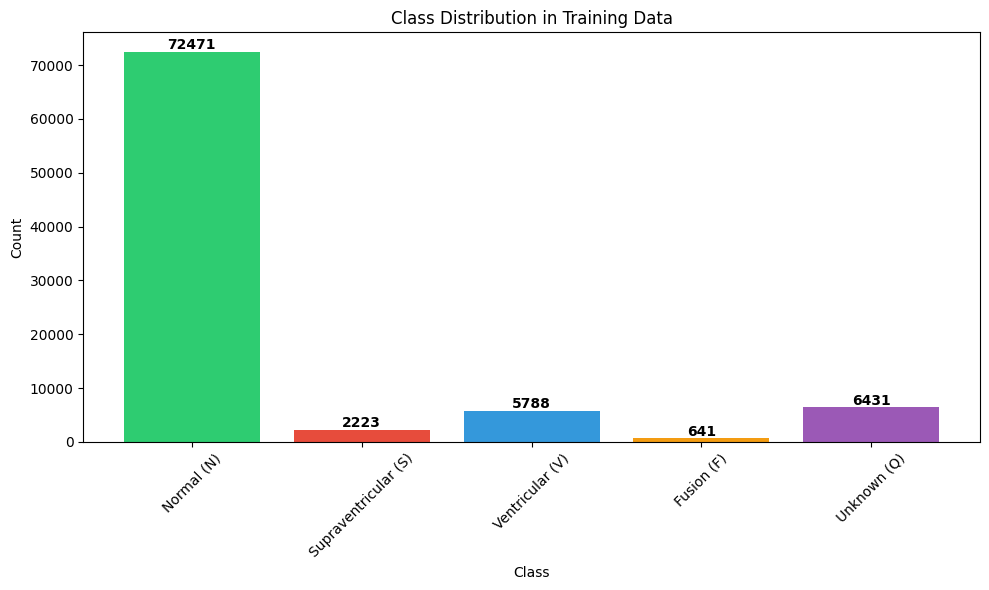
\includegraphics[width=\columnwidth]{figures/class_distribution.png}
\caption{Class distribution in the training dataset showing significant imbalance between normal beats and various arrhythmia types.}
\label{fig:class_distribution}
\end{figure}

\begin{figure}[H]
\centering
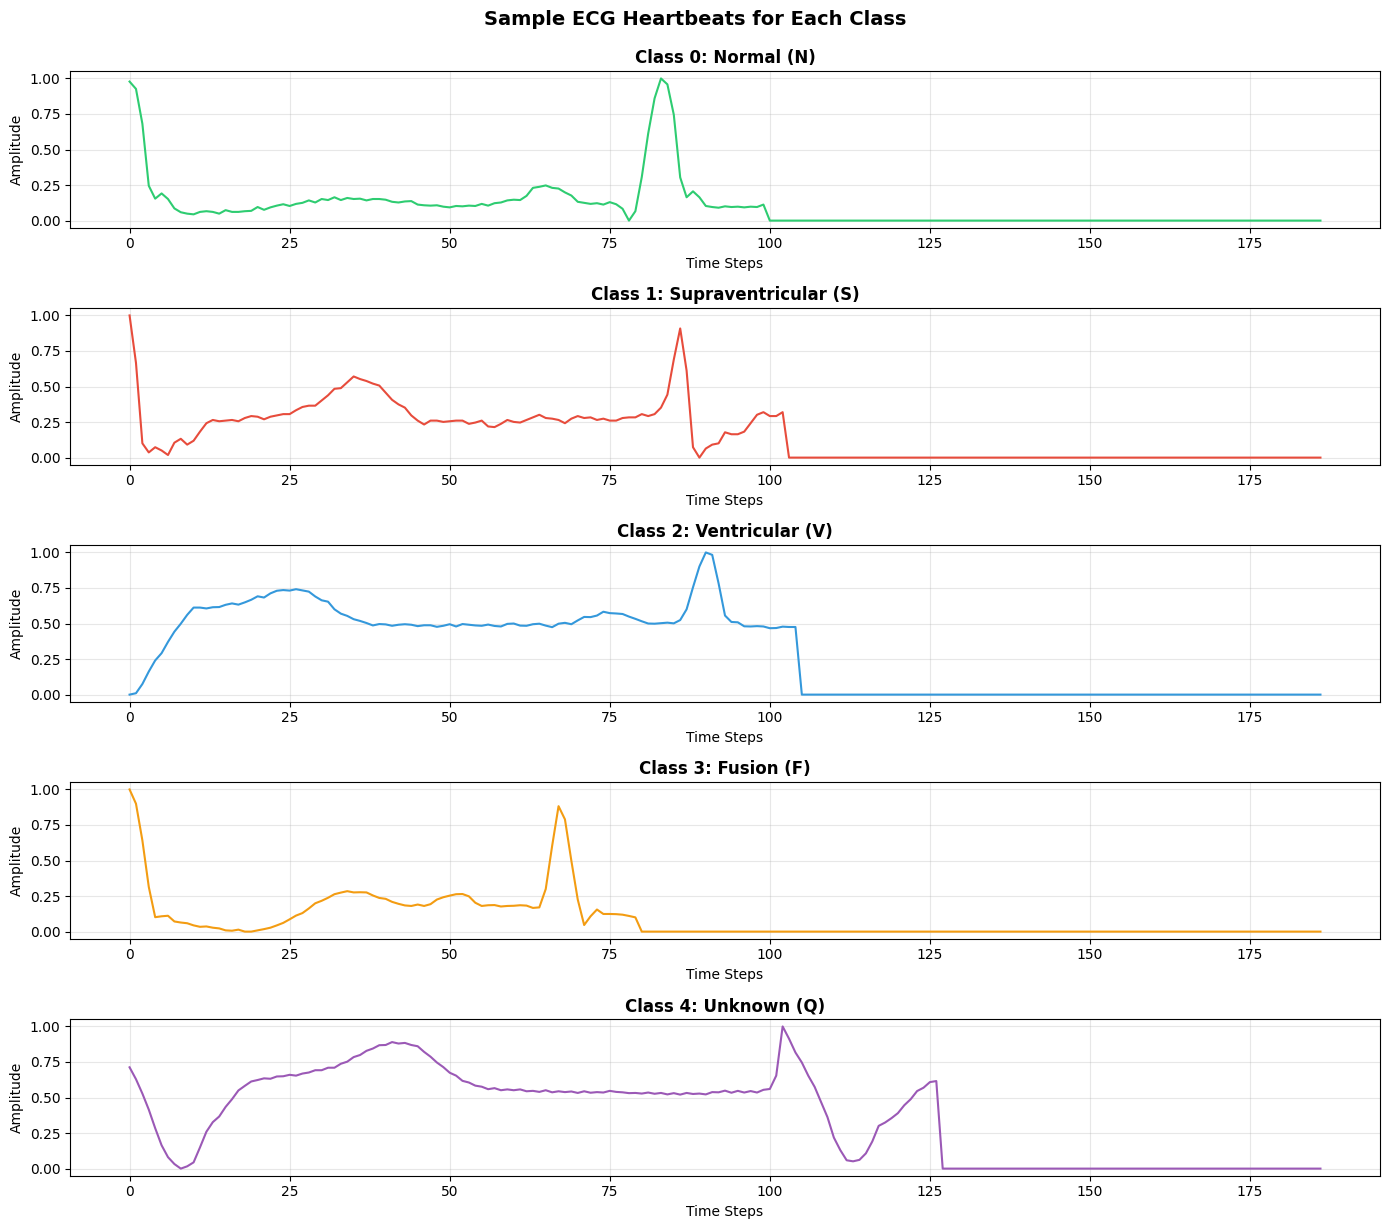
\includegraphics[width=\columnwidth]{figures/ecg_samples.png}
\caption{Representative ECG heartbeat signals for each of the five classes: (a) Normal, (b) Supraventricular, (c) Ventricular, (d) Fusion, and (e) Unknown beats.}
\label{fig:ecg_samples}
\end{figure}

\begin{figure}[H]
\centering
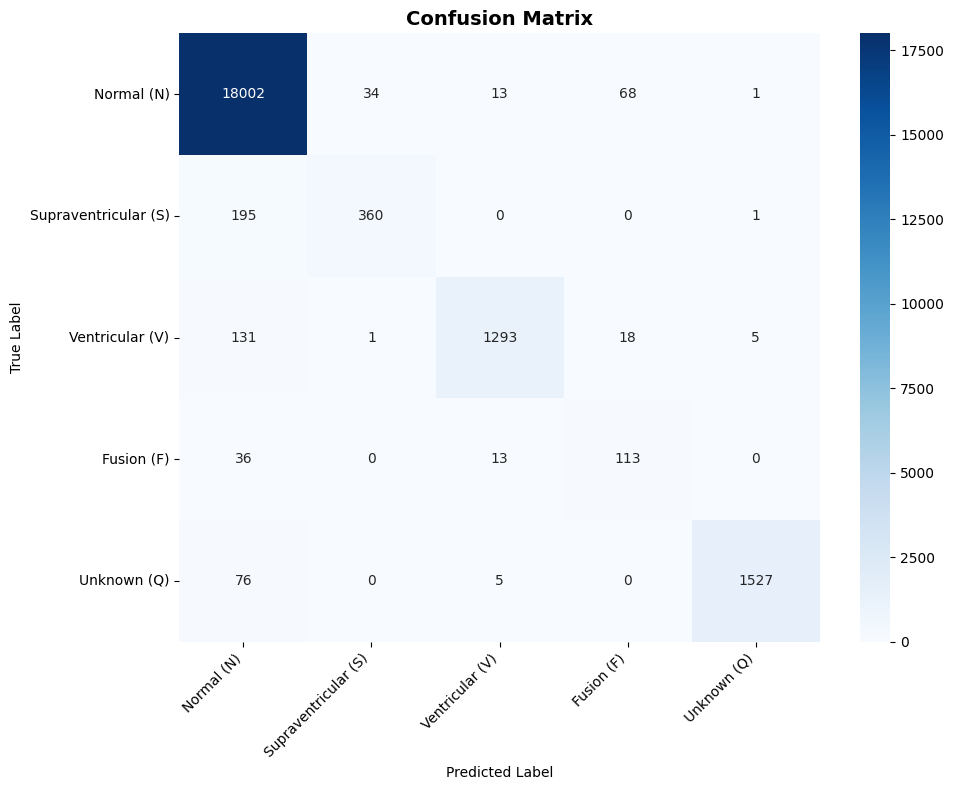
\includegraphics[width=\columnwidth]{figures/confusion_matrix.png}
\caption{Confusion matrix showing the classification performance across all five heartbeat classes.}
\label{fig:confusion_matrix}
\end{figure}

\begin{figure}[H]
\centering
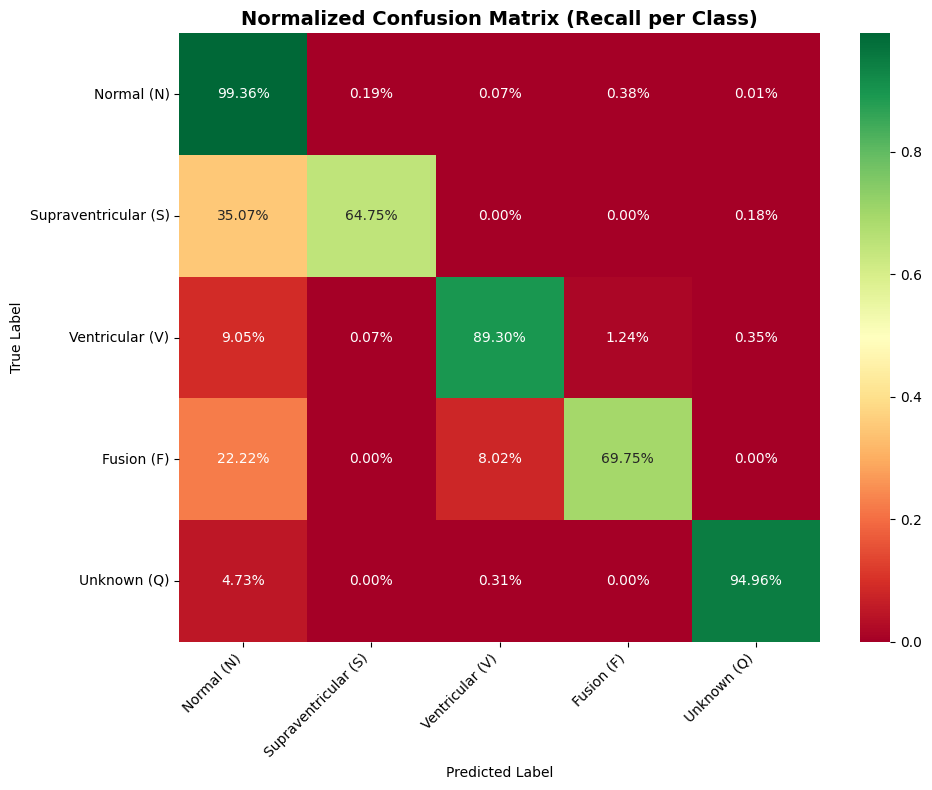
\includegraphics[width=\columnwidth]{figures/confusion_normalized.png}
\caption{Normalized confusion matrix displaying recall (sensitivity) for each class as percentages.}
\label{fig:confusion_normalized}
\end{figure}

\begin{figure}[H]
\centering
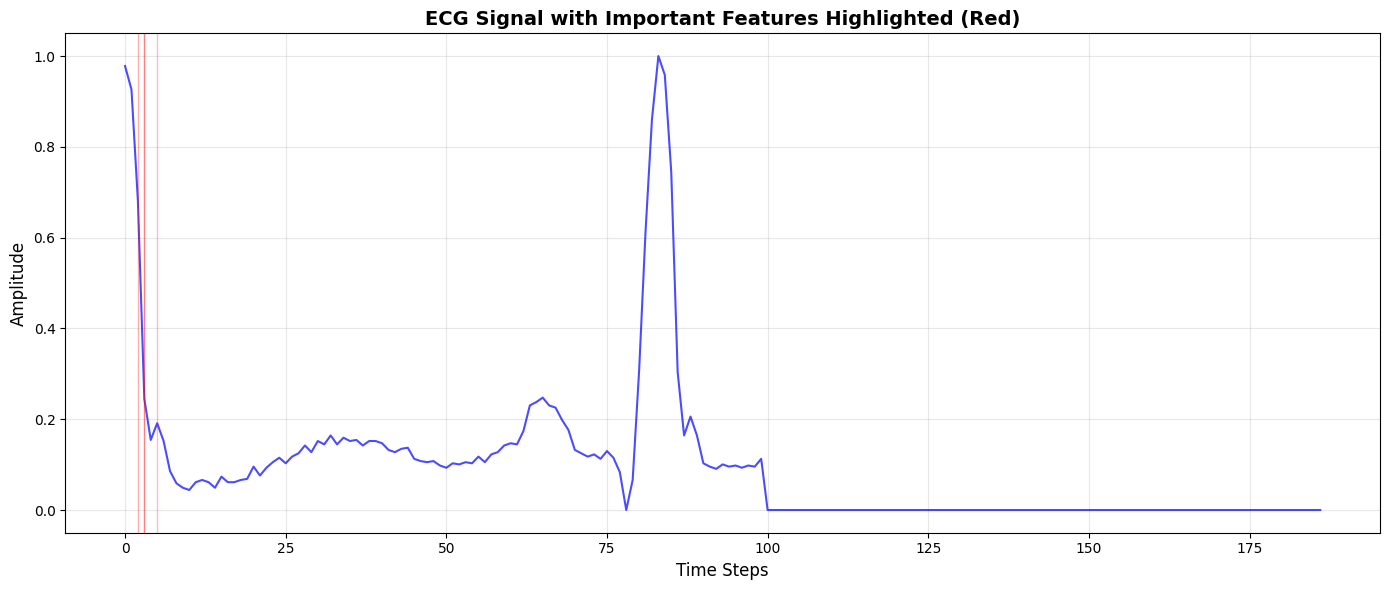
\includegraphics[width=\columnwidth]{figures/feature_importance.png}
\caption{Top 30 most important time steps (features) in the ECG signal for classification, ranked by importance score.}
\label{fig:feature_importance}
\end{figure}

\section*{Acknowledgment}

The authors acknowledge the use of the MIT-BIH Arrhythmia Database, which is a widely recognized benchmark dataset for ECG signal analysis research.

\end{document}



